\chapter{Interpretation for the Seesaw Model}
\label{sec:Interpretation}
\label{sec:Interpretation/Seesaw}

As no statistically significant excess was observed, we calculate expected and observed upper limits on the cross section sum for the production of seesaw heavy fermion pairs ($\Sigma^0\Sigma^+$, $\Sigma^0\Sigma^-$, or $\Sigma^+\Sigma^-$), assuming a flavor-democratic value for the mixing angle parameters, $V_e = V_\mu = V_\tau = 10^{-6}$, and degenerate heavy fermion masses $m_\Sigma$. The calculation is done using asymptotic CL$_s$ limits with a confidence level of 95\,\% \cite{Junk:1999kv,Read:2000ru,Read:2002hq}.
%Taking the ratio of the cross section upper limit and the signal cross section, one obtains the so-called $r$-value which indicates whether the signal at hand is excluded ($r < 1$) or cannot be excluded ($r > 1$).

If the data agreed perfectly with the background estimates, we would expect our analysis to exclude type-III seesaw heavy fermion pair production for masses below $m_\Sigma = 430\,\GeV$. The observed limit is at 435\,\GeV. While it lags the expected value, the difference is within the uncertainty range because the event category that shows apparent excess as discussed above is not very sensitive to the seesaw signal (Fig.~\ref{fig:Results}a). The full exclusion curve is shown in Fig.~\ref{fig:exclusion}.

\begin{figure}[t]
\begin{center}
	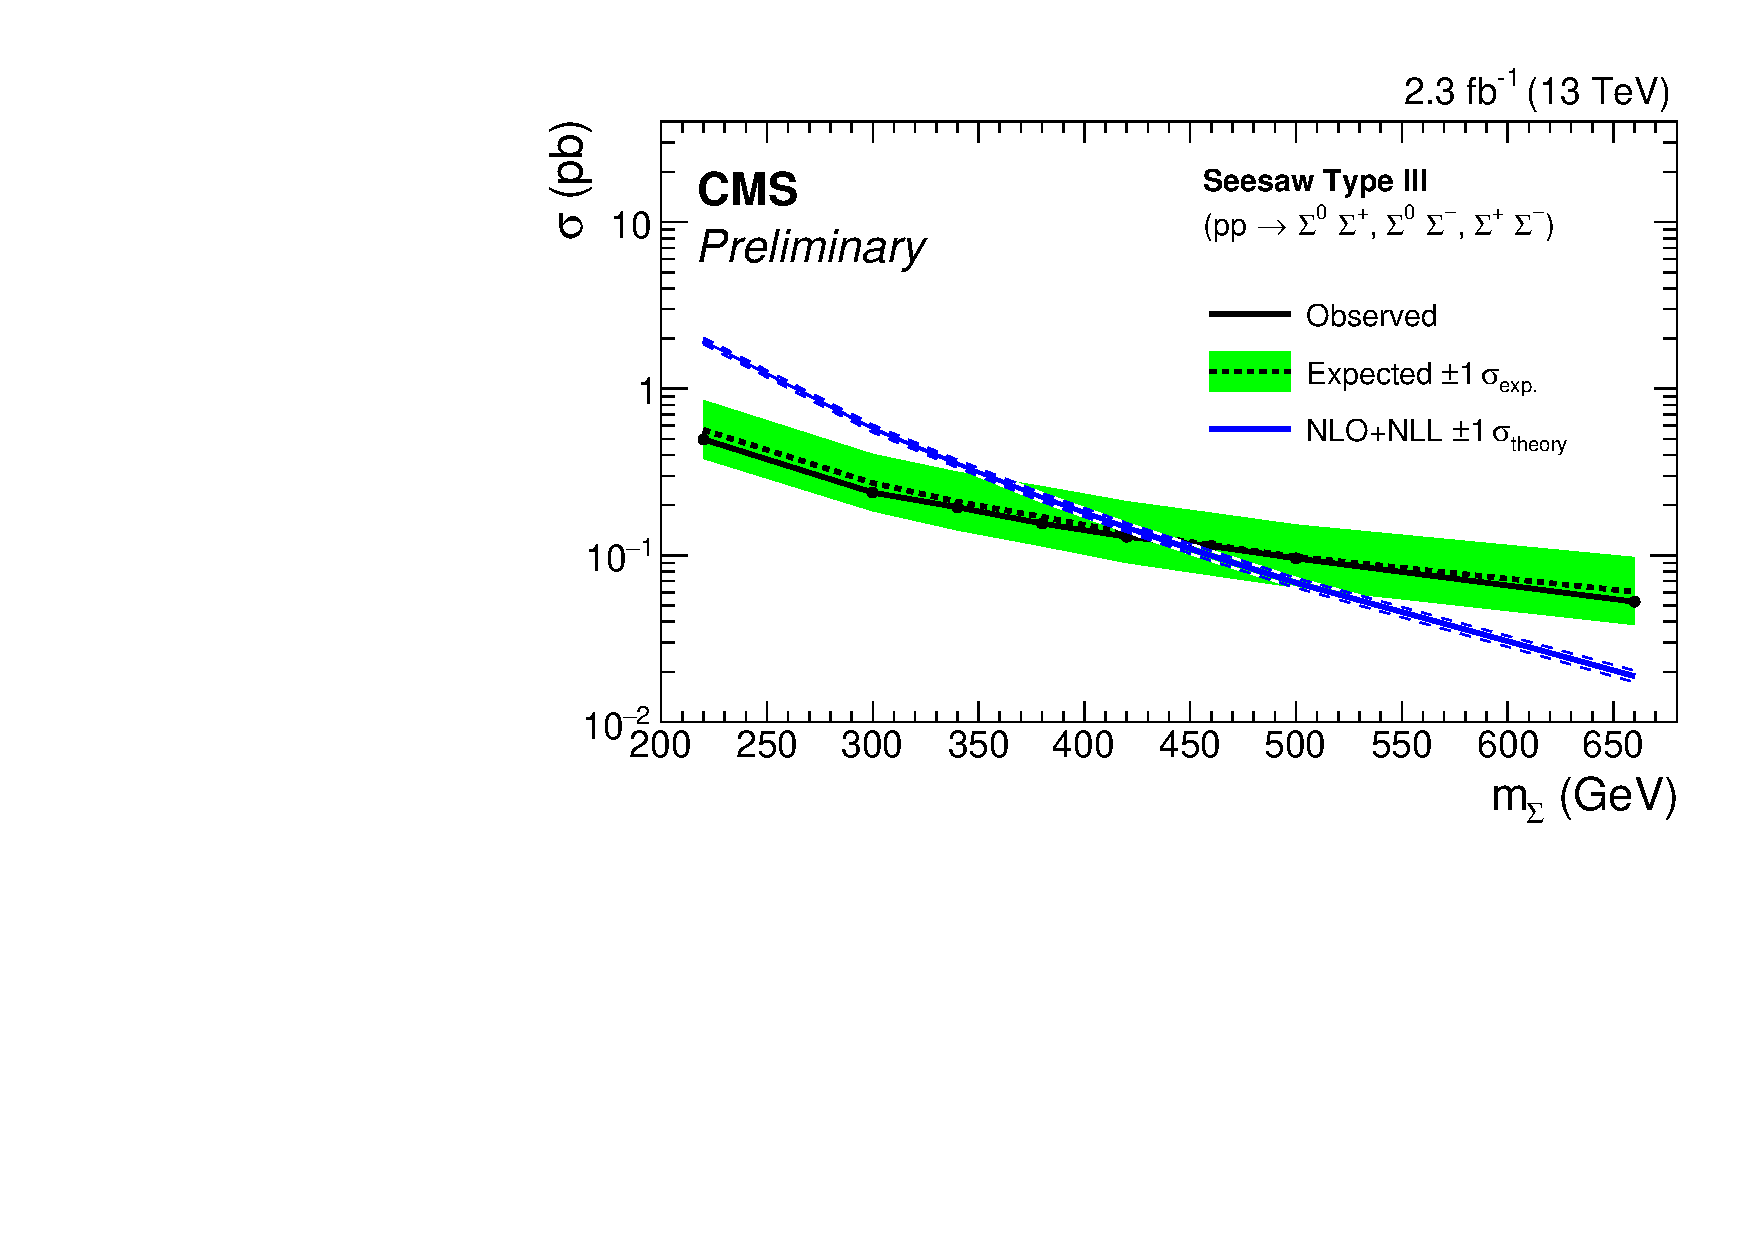
\includegraphics[width=.8\textwidth]{Interpretation/exclusion}
	\caption{Exclusion for the flavor-democratic type-III seesaw model ($V_e = V_\mu = V_\tau = 10^{-6}$). We exclude heavy fermion pair production for masses below $m_\Sigma = 435\,\GeV$ (expected: 430\,\GeV) and give upper limits on the pair production cross section.
	\label{fig:exclusion}}
\end{center}
\end{figure}

In comparison to the Run-I results, the search sensitivity has been enhanced by various improvements, most notably the inclusion of new decay modes involving the Higgs boson and of 4-lepton channels, and by the introduction of an improved fine-grained binning scheme. Exclusion limits from the CMS Run I result were at $m_\Sigma = 250\,\GeV$ (expected) and $m_\Sigma = 278\,\GeV$ (observed) \cite{CMS-PAS-EXO-14-001}.
